\chapter{Introduction to XBee}

One of the main characteristics of WSNs is the ability each node has to wirelessly communicate with other nodes. 
During this course will be doing this with ZigBee protocol compliant radios, like XBee~\cite{faludi2010bws}.

Throughout this section you will be introduced to the different components and code that will allow you to set a basic wireless network with XBee modules.

\section{The XBee module hardware configuration}\label{xbee:hardware}

Xbee modules come in different configurations. The one we will be using is called XBee-Series 2 with wire antenna and it is shown in Figure~\ref{fig:xbee}.

\begin{figure}[htbp]
  \centering
  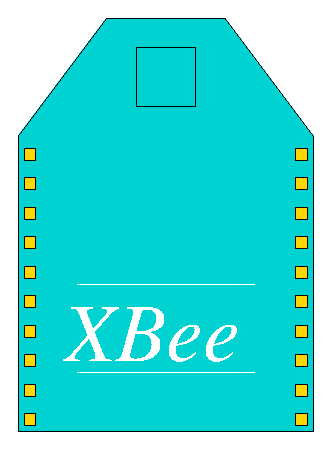
\includegraphics[width=0.4\linewidth]{figures/xbee.eps}
  \caption{XBee Series 2 with wire antenna
  \label{fig:xbee}}
\end{figure}

This device supports different kinds of ZigBee in mesh networking. Its wire antenna provides omnidirectional coverage, or what is the same as saying that its coverage is pretty much the same in all directions when the antenna is straight and perpendicular to the module.

If you flip the XBee, you will be able to see the pins through which it can send/receive data to/from sensors, comunicate with Arduino, connection to a power supply and GND (more information about the pins can be found in page 15 of~\cite{faludi2010bws}).

\subsection*{Comunicating with the XBee}

We can access and program de XBee through any terminal application and a USB connection. The breakout board shown in Figure~\ref{fig:breakoutBoard} allows us to: $1$) plug the XBee into a breadboard, facilitating the wired connections with other componentes (including the Arduino); as well as the ability to $2$) stablish a USB connection to configure the XBee.

\begin{figure}[htbp]
  \centering
  \includegraphics[width=0.4\linewidth]{figures/breakoutBoard.eps}
  \caption{XBee Explorer board from SparkFun
  \label{fig:breakoutBoard}}
\end{figure}

As the pins on the XBee are separated differently than the holes in the breadboard, everytime a configuration or wired connection is needed, the XBee should be placed in the breakout board as shown in Figure~\ref{fig:xbeeAndBreakoutBoard}, and then placed on the breadboard.

\begin{figure}[htbp]
  \begin{center}$
    \begin{array}{cc}
      \includegraphics[width=0.4\linewidth]{figures/xbeeAndBreakoutBoard.eps}\label{xbeeOutside} &
      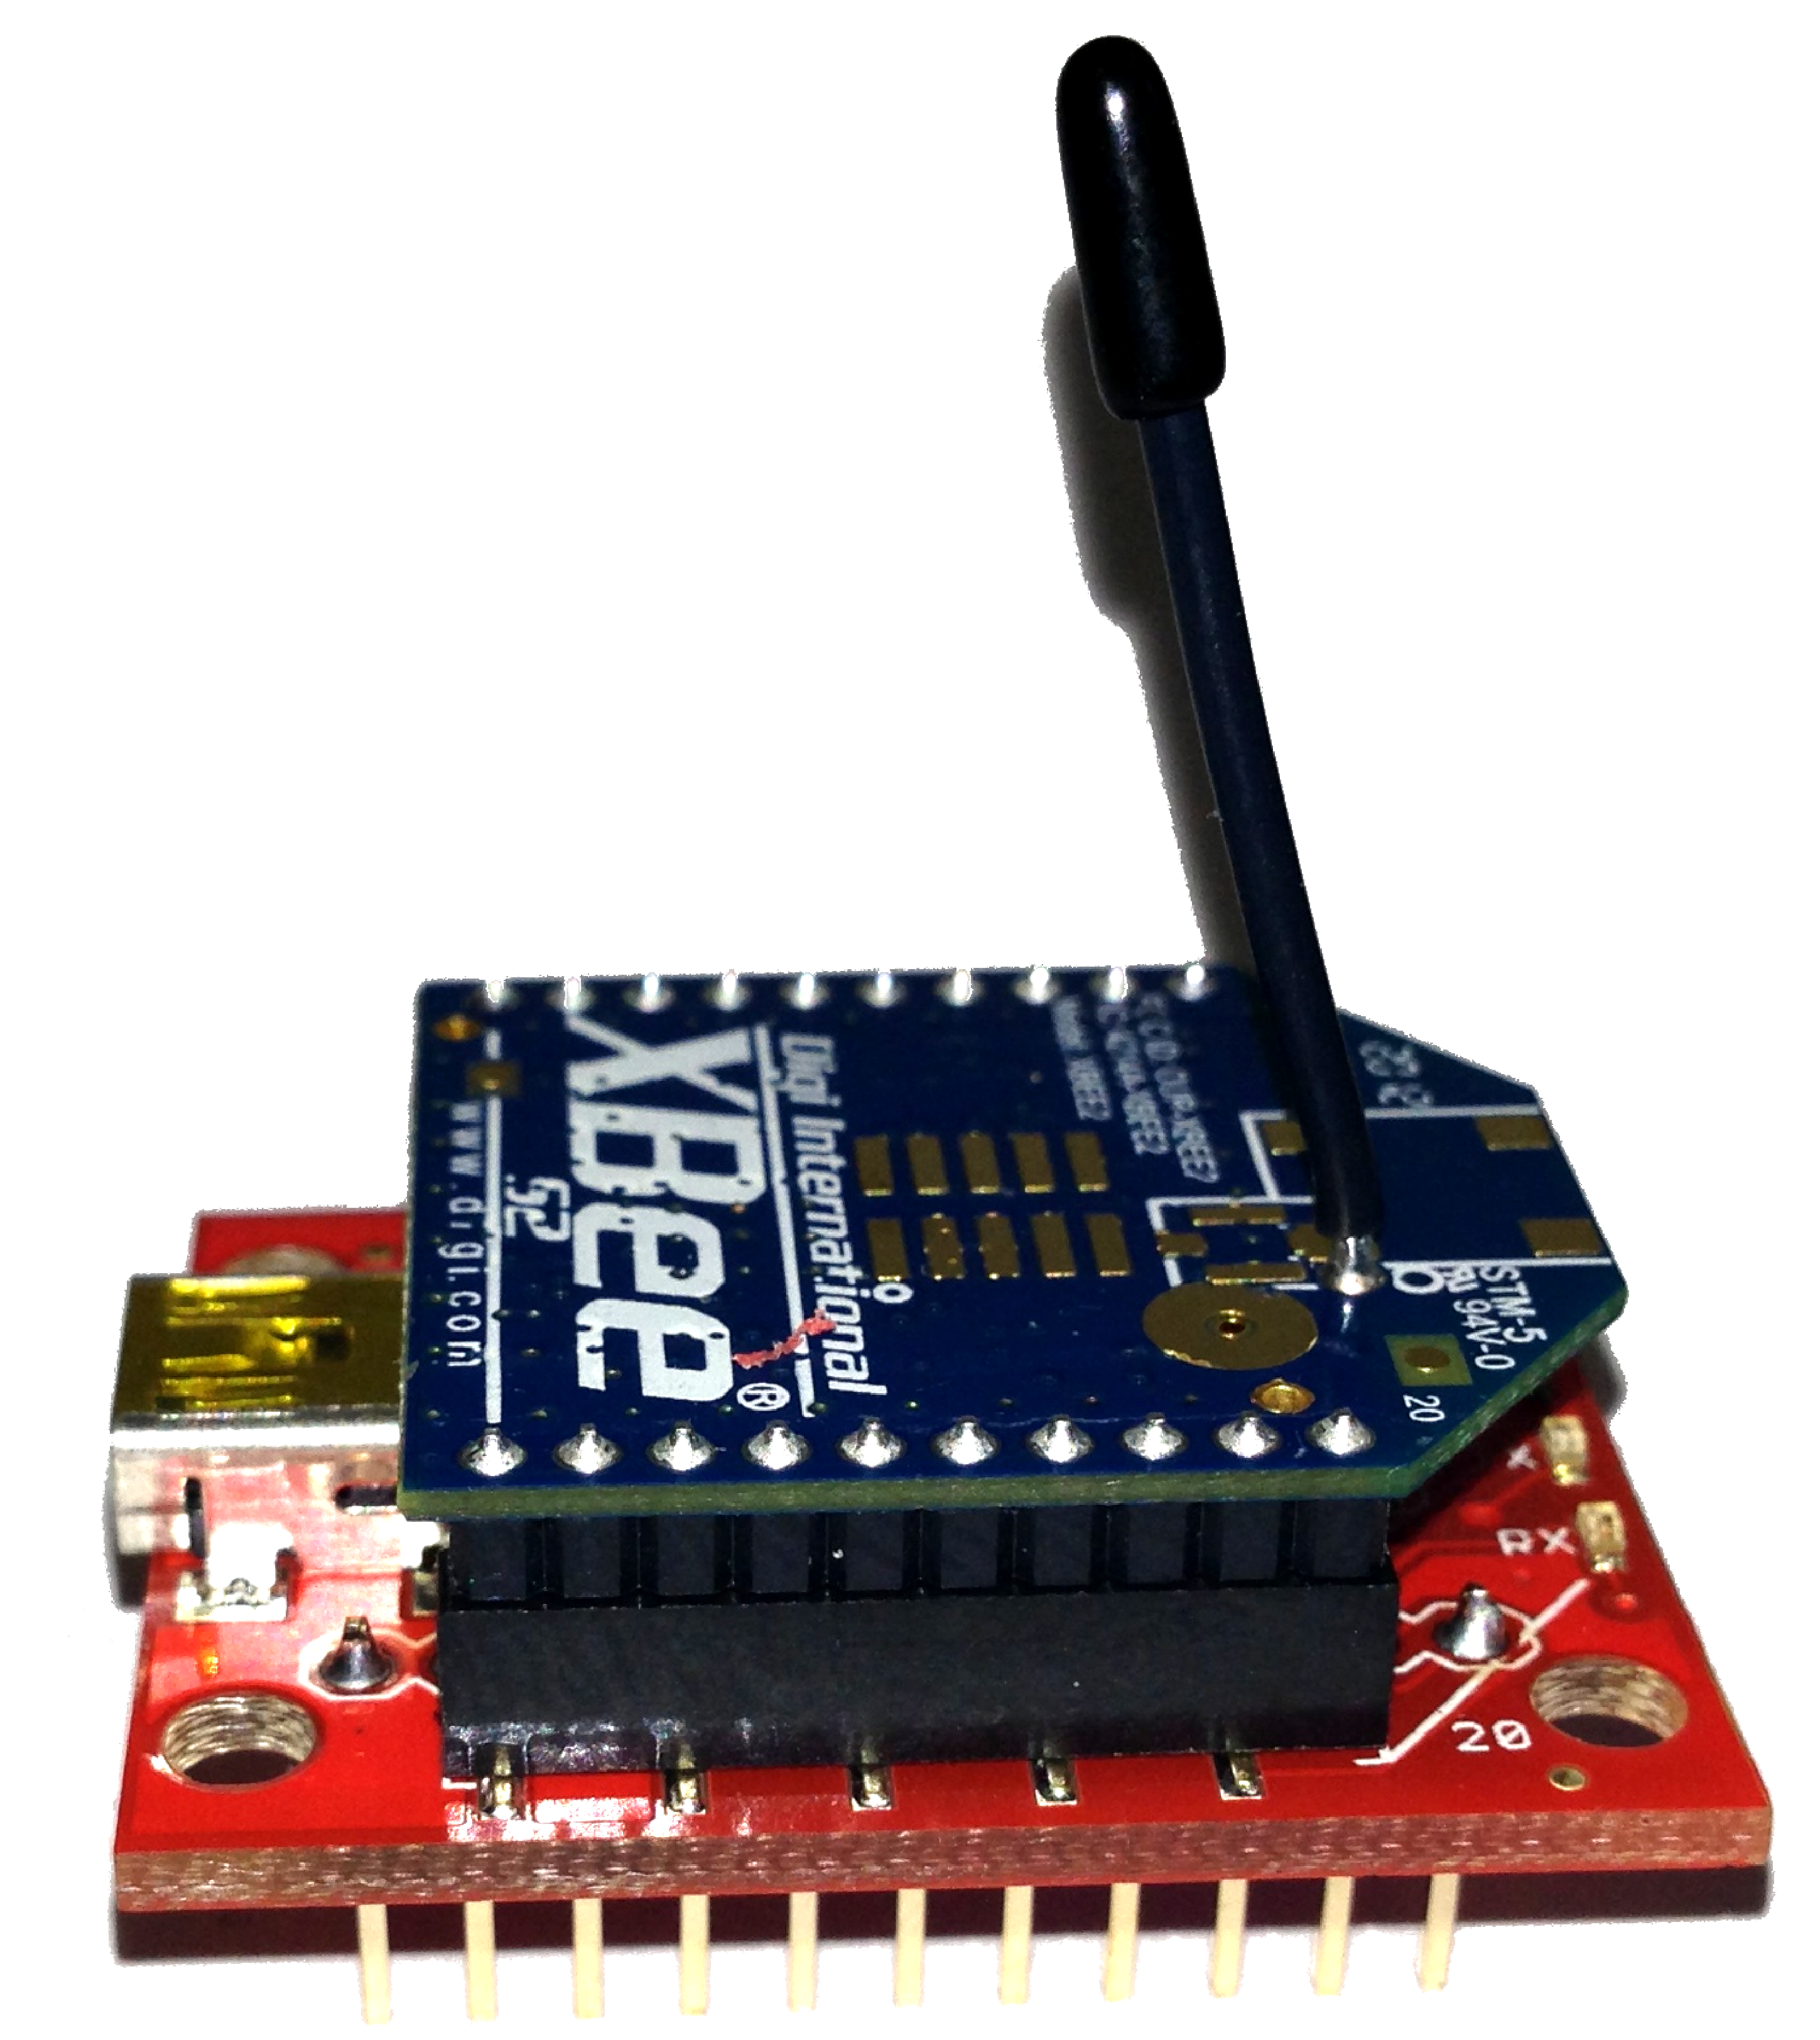
\includegraphics[width=0.4\linewidth]{figures/xbeeAndBreakoutBoard-inserted.eps}\label{xbeeInside}
    \end{array}$
  \end{center}
  \caption{XBee and breakout board: Left: Xbee outside; see the different spacing of the pings. Right: Xbee inside; setup for configuring and pluging into breadboard.
    \label{fig:xbeeAndBreakoutBoard}}
\end{figure}

